\documentclass[runningheads]{llncs}

\usepackage[T1]{fontenc}

\usepackage{cite}
\usepackage{graphicx}
\usepackage{amsmath}
\usepackage{float}
\usepackage{enumitem}
\usepackage[linesnumbered,ruled,vlined]{algorithm2e}

\setlistdepth{3}
\setlist[enumerate,1]{label=\textbf{\arabic*.}, ref=\arabic*}
\setlist[enumerate,2]{label=\textbf{\theenumi.\arabic*.}, ref=\theenumi.\arabic*}
\setlist[enumerate,3]{label=\textbf{\theenumii.\arabic*.}, ref=\theenumii.\arabic*}

\bibliographystyle{plain}
\begin{document}

\title{Natural Deduction Proofs for Educational Feedback}

\author{Daniel Macau\inst{1}
\and Ricardo Gonçalves\inst{1}
\and João Costa Seco\inst{1}}

\institute{NOVA School of Science and Technology, Caparica, Portugal}

\maketitle 

\begin{abstract}
Online tools, where students can practice and have automatic feedback, have shown to be useful both for MOOCS or as complementary material for traditional classes. Nevertheless, contrary to the myriad of tools that exist for learning programming languages, in the area of logic, a fundamental subject in any Computer Science programme, there is still a lack of such online tools, and in particular for the challenging exercise of Natural Deduction (ND) proofs. The few existing tools usually do not provide effective feedback, which is in fact challenging since tree-like ND proofs are non-linear and some steps are not immediate, as it is the case of proofs by contradiction. In this paper, we present an algorithm for pedagogical purposes that can generate human-readable ND proofs for a given problem. The algorithm supports both Propositional and First-Order Logic, and is based on directed hypergraphs. This allows obtaining the shortest and most direct proof for a given problem, but it can also adapt to a user’s current unfinished proof, allowing for greater flexibility in the proof construction. The algorithm can be integrated with educational platforms to guide users through the proofs by providing advanced feedback, at the same as it can help teachers grading ND exercises. 

\keywords{Natural Deduction  \and Propositional Logic \and First Order Logic \and Automation \and Algorithm \and Feedback \and Grading}
\end{abstract}

\section{Introduction}
Learning logic is a fundamental component of today’s curriculum, as it plays a key role in several important areas, including programming languages, databases, artificial intelligence, and algorithms~\cite{logicincomputer}. Logic courses cover a wide range of topics, and one that stands out is ND, given its importance in helping students develop reasoning skills~\cite{autogeneratingnd}, which are valuable in real-world contexts where structured thinking and argumentation are required~\cite{vonPlato_2014}.

Natural deduction exercises are generally considered among the most challenging for students due to the complex reasoning involved. Since mastering them requires extensive exposure, many students struggle to become familiar with the rules and the formal way of thinking. These exercises involve numerous logical rules, and it is not always clear which one to apply. Additionally, students often need to keep track of multiple steps and assumptions simultaneously, which can be confusing.

Despite the importance of logic education, there remains a lack of online tools that support this type of exercise. The few existing tools typically offer very limited feedback, focusing mainly on syntactic and semantic errors while failing to provide deeper guidance that could help students overcome conceptual difficulties~\cite{Perh__2025}. A major challenge students face when solving ND problems is becoming stuck either because they reach an impasse or feel they are overcomplicating the exercise.

This highlights the need for more advanced and effective feedback systems to address these gaps. One approach to producing this type of feedback is through algorithms capable of generating complete proofs. This allows the system to derive hints from the generated proof, ensuring that the guidance leads to a correct solution rather than a dead end. However, most existing algorithms were not developed for this purpose: while they can find a solution or detect contradictions, they often lack flexibility in terms of rule application, depend on the specific ND system used, and cannot dynamically adapt to a user’s reasoning process. Capturing the user’s reasoning enables the feedback to be personalized and aligned with the student’s chosen path.

In this article, we present an algorithm developed during a thesis project with a pedagogical focus. It was originally created to support an application that helps students build and verify ND proofs. However, the application itself is not addressed in this article.  The algorithm is capable of automatically generating multiple Gentzen-style proofs for the same problem in a human-readable way, both in PL and FOL. A distinguishing feature of our algorithm is its ability to adapt to a user’s solution, providing step-by-step guidance that aligns with the student’s reasoning process. This is made possible through the use of directed hypergraphs that store information about which rules can be applied at each step, capturing multiple valid proof paths. By leveraging well-known graph search and traversal algorithms, the system not only finds correct solutions but also identifies the shortest proofs, enabling feedback on how a solution could be improved. Additionally, the algorithm can be used to assess exercises by determining how far a student’s resolution is from a valid or optimal solution, thereby offering a measurable assessment of proofs.

\section{Related Work}
Several algorithms have been developed to verify the validity of logical formulas. One common approach is to use resolution to find contradictions. This method begins by converting formulas into Conjunctive Normal Form, which is easier for automated systems to process. After this transformation, the algorithm applies resolution rules to search for contradictions. If a contradiction is found, the formula is not valid. If no contradiction appears after checking all possible combinations, the formula is considered valid. However, this method often does not produce proofs that are easy for humans to understand.
To address this, David Robinson~\cite{robinson_using} proposed an algorithm that uses a version of resolution compatible with natural deduction. His method works by encoding formulas into special clauses and then using resolution steps to reconstruct a natural deduction proof. The result is a proof that is easier for people to read and understand.
Another approach is the algorithm developed by Xuehan Maka Hu~\cite{makahu_automatic}. This algorithm works by recursively applying introduction rules to break down the conclusion, and then using elimination rules to handle the assumptions. It generates complete and human-readable natural deduction proofs in Gentzen style for propositional logic. Although it produces understandable proofs, the algorithm is not very flexible. Its strict rule application can sometimes lead to complicated solutions for problems that could be solved more simply.

Bolotov's~\cite{bolotov_2005_automated} algorithm is another example of a proof-searching method designed for natural deduction in propositional logic. It follows a goal-directed strategy, combining forward and backward rule applications. It updates the goals dynamically and stops when a proof is found or when no further progress is possible, returning a counter-example in the latter case. One limitation of this algorithm is that it does not include a mechanism to remove irrelevant or unnecessary branches during proof search. These extra branches may contain valid but unneeded steps, which can make the proofs longer and harder to follow.
LOGAX~\cite{lodder_2020_generation} is an interactive tutoring tool that constructs Hilbert-style axiomatic proofs in propositional logic. It is designed to provide students with step-by-step hints and feedback. LOGAX uses a version of Bolotov's algorithm to generate directed acyclic multigraphs, which allow the system to store and explore multiple proof paths for the same problem. It can adapt the proof it generates to match the student's reasoning, offering both forward and backward hints depending on the student's progress. Despite its strengths, LOGAX has some limitations. It is only designed for propositional logic and can only generate linear Hilbert-style proofs. Since it is based on Bolotov's algorithm, it also inherits some of its weaknesses, including the possibility of generating longer proofs with irrelevant or unnecessary steps.

The algorithm proposed by Ahmed, Gulwani, and Karkar~\cite{IJCAI13} uses a very similar approach to our algorithm but is applied to a different set of inference rules and only works for PL. It is based on a hypergraph called the Universal Proof Graph (UPG), where nodes represent possible formulas (they are represented as bitvectors that map each formula to a truth table, reducing the number of formulas in the graph for better performance), and the edges represent possible rule applications that can be applied under each node. From that graph, we can extract abstract proofs (called "abstract" because expressions are still mappings to truth tables and not actual formulas), which are later converted into natural deduction proofs. The algorithm can also be used to generate problems and specify their difficulty, which can be useful for teachers. A big problem the algorithm faces is that it can only solve PL problems, since we cannot map FOL expressions to truth tables. Another issue is related to proof size, as the algorithm cannot guarantee that the solution found is the smallest one within the space explored.

\section{Natural Deduction}

ND is a logical proof system that reflects mathematical and everyday reasoning under assumptions~\cite{nd-mancosu}. It emerged in 1934 with Gentzen and Jaśkowski's work, gaining widespread acceptance by the 1960s~\cite{Pelletier1999-FRAABH}. Using ND, an important goal is to verify whether a formula \(\varphi\) is a semantic consequence of a set of formulas \(\Gamma\), written \(\Gamma \vdash \varphi\). This means that whenever all formulas in \(\Gamma\) hold, \(\varphi\) must also hold because it logically follows from \(\Gamma\) \cite{gouveia_lgica1, gouveia_lgica2}. There are many ways to represent these proofs. The two main styles that exist are the Gentzen style, which organizes the proof in a tree-shaped structure, and the Fitch style, which uses a linear structure with deeper indentation levels to represent assumptions or intermediate steps in the proof. Our article focuses on the first one. 

Gentzen style uses tree-shaped structures, also known as deduction trees. These structures represent proofs and are built by starting with individual trees, which are formulas, and successively applying rules of inference to generate new and more complex trees. The formula at the root is the conclusion of the proof, and formulas at the leaves are called hypotheses and are generally associated with marks. In this article, we use numbers to denote such marks. Marks are used to identify distinct assumptions and to indicate when they are discharged (closed). A hypothesis is considered discharged if its mark is referenced by a rule. Rules are represented using fractions (a horizontal line), where hypotheses appear above the line and the rule’s conclusion appears below. The rule’s name and the marks for the hypotheses are normally placed on the right-hand side of the fraction. There are two main groups of rules for each logical connective: introduction (\(I\)), which constructs more complex formulas from simpler ones, and elimination (\(E\)), which extracts information from complex formulas. Additionally, a special rule, known as absurdity (\(\bot\)), allows deriving any conclusion from a contradiction. Each rule has its own characteristics, and some can only be applied under specific circumstances, called side conditions. For simplicity, we do not discuss these here, but they are included in our algorithm. Figure \ref{fig:nd-rules}, list all the rules considered in our implementation. Greek letters represent generic formulas. The symbols \( \mathcal{D} \) represent subtrees within branches, while \( m \) and \( n \) denote marks. The notation \(\displaystyle \left[ \varphi \right]^a_{\substack{b}}\) indicates the substitution (or mapping) of terms from \( a \) to \( b \), and \(\displaystyle [\varphi]^m\) represents which assumptions can be used in each branch by the rule.

\begin{figure}
    \centering
    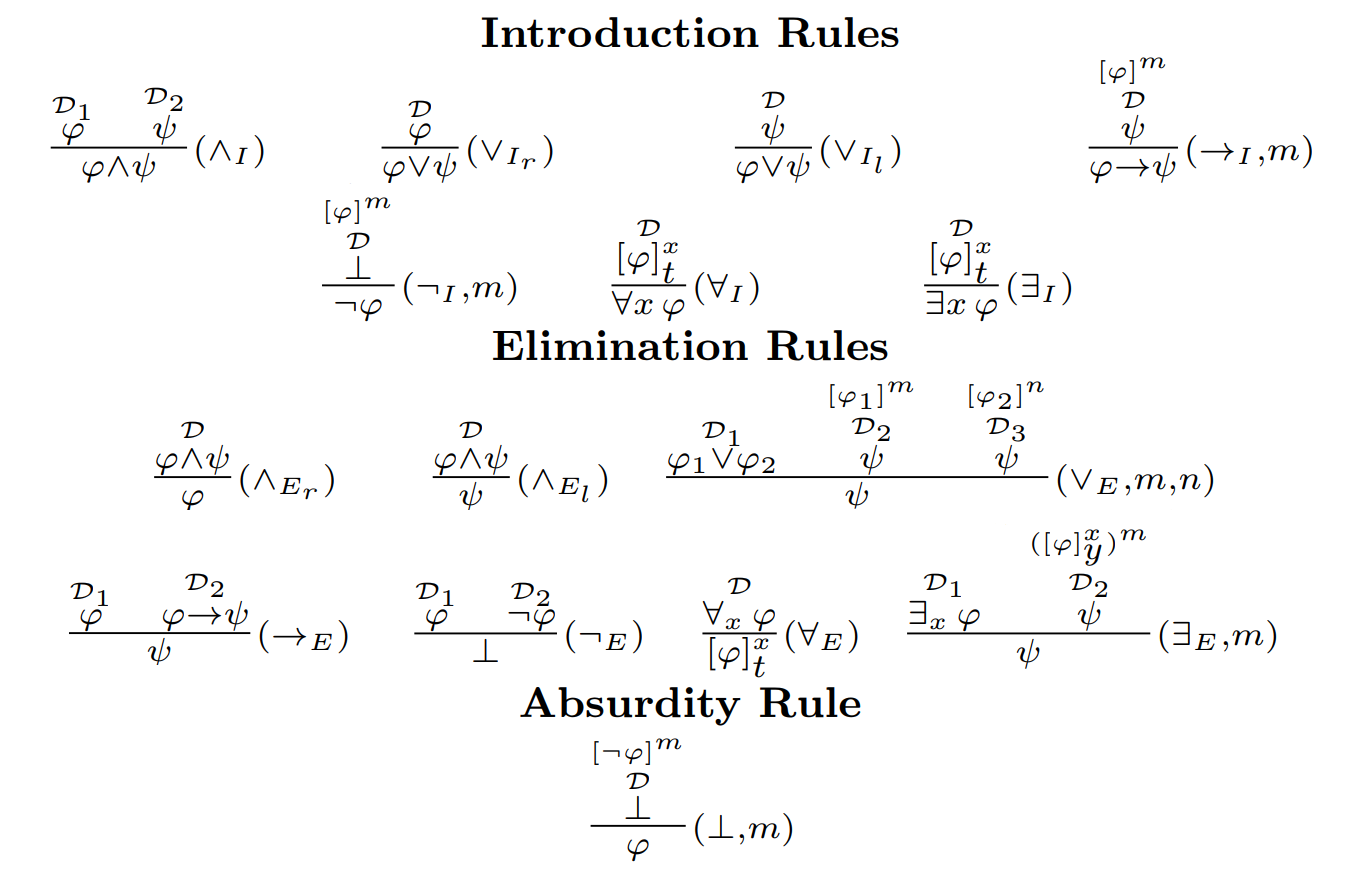
\includegraphics[width=1\linewidth]{resources/rules.png}
    \caption{List of rules for both PL and FOL}
    \label{fig:nd-rules}
\end{figure}

These proofs can be constructed either bottom-up, from the conclusion to the hypotheses, or top-down, from the hypotheses to the conclusion. Figure \ref{tab:proof-tree} shows an example of a proof, that solves the problem: \( \vdash \neg (\varphi \lor \psi) \to \neg \psi \).

\begin{figure}
    \centering
    \[
    \frac{\displaystyle \frac{\displaystyle \frac{
    \displaystyle \neg (\varphi \lor \psi)^1 \quad \displaystyle \frac{\psi^2}{(\varphi \lor \psi) \strut} \quad (\lor_{I_l}) \strut}
    {\displaystyle \bot \strut} \quad (\displaystyle \neg_E)\strut} {\displaystyle \neg \psi \strut} \quad (\neg_I, 2) \strut}
    {\neg (\varphi \lor \psi) \to \neg \psi \strut} \quad (\to_I, 1)
    \]
    \caption{Tree proving \( \vdash \neg (\varphi \lor \psi) \to \neg \psi \).}
    \label{tab:proof-tree}
\end{figure}


\begin{definition}[Well-Formed Tree Proof]
A tree proof is well-formed if and only if it is finite and applies the inference rules correctly.
\end{definition}

\begin{definition}[Tree Proof Correctness]
Given a tree proof and a problem \(\Gamma \vdash \phi\), we say that the tree solves the problem if and only if it is well-formed and both of the following conditions hold:
\begin{enumerate}
    \item The root of the tree is \(\phi\).
    \item Every open hypothesis in the tree is contained in \(\Gamma\).
\end{enumerate}
\end{definition}

\section{Algorithm}
Developing an algorithm to provide advanced feedback on ND exercises begins with clearly defining its key features. Our goal was to design an effective feedback system capable of delivering relevant information to assist students in solving proofs, making the learning process more teaching-like and adapted to each student’s resolution. With this focus, we identified four fundamental aspects of a well-designed feedback system:

\begin{itemize}

\item \textbf {Providing guidance on rule applications:} Some rule applications in ND are not obvious, making it difficult for students to progress. For example, sometimes, no matter how hard students try, the desired proof cannot be obtained. This may be because an indirect proof is needed: a sentence \(\varphi\) is proved by assuming \(\neg \varphi\) and showing that it leads to a contradiction [NDpack]. The system should be able to identify such situations and suggest the appropriate rule applications.

\item \textbf {Breaking proofs into smaller sub-proofs:} To simplify reasoning, the feedback should allow students to focus on smaller proofs. By dividing proofs into smaller steps, it will reduce the cognitive load and encourage incremental learning. 

\item \textbf{Indicating the distance to a solution:} Showing how many steps (rule applications) are needed to complete the proof helps students maintain focus and gain a clear sense of progress.

\item \textbf{Improvements in the proof:} Providing feedback about irrelevant steps taken or possible shortcuts that the student could apply to make the proof clearer. This can also be used to show different ways to tackle the same problem.

\end{itemize}

These components offer several advantages in the learning process. By providing structured and clear information, the system becomes more robust, helping students overcome challenges throughout the proof.

\section{Procedure}
In this chapter, we explain how our algorithm was built. The algorithm is divided into three sequential steps. 
The main idea of our algorithm is to first generate a hypergraph based on the input problem and the part of the proof we want to complete. This graph stores all the possible rule applications for that problem. Then, we use this graph to build a second hypergraph that tries to simulate as many proof constructions as possible. In the last step, we trim this second graph so that it keeps only the proofs that solve the problem. Then, we can use the resulting graph to extract and build proofs, which can later be used to generate feedback. For the sake of simplicity, we only cover the PL implementation, but the same procedure can be applied to FOL with some adjustments.

\subsection{Transition Graph}
The first step is to build the Transition Graph (TG). For that, we need the problem we want to solve and, in the cases where we want to complete a proof and provide a personalized solution, the initial state from which we want to start generating the solution. In other words, it represents the part of the proof that needs to be completed. The state is extremely important in this stage because it is where the algorithm considers the differences between the student's incomplete solution and the actual solution of the problem. Before we describe the procedure, let us introduce some definitions:

\begin{definition}[State]
A state is defined as a pair:
\[
S = (\alpha, \Delta)
\]
where \(\alpha\) is the formula, and \(\Delta\) is the set of hypotheses, including both premises and any assumptions made up to that point in the proof.
\end{definition}

For example, the problem itself can be seen as a state \(S = (\varphi, \Gamma)\). In Figure \ref{tab:proof-tree}, the root has the state \(S_{\text{root}} = \big(\neg (\varphi \lor \psi) \to \neg \psi, \emptyset \big),\) and the leaves have the states 
\( S_{\text{left}} = \big(\neg (\varphi \lor \psi), \{\neg (\varphi \lor \psi), \psi\}\big)\) and \(S_{\text{right}} = \big(\psi, \{\neg (\varphi \lor \psi), \psi\}\big)\). For FOL proofs, we also need to consider the side conditions up to that state.

\begin{definition}[Transition Graph]
The TG is defined as a triple:
\[
TG = (F, R, E_T),
\]
where \( F \) is a finite set of possible logical formulas that our solutions can have, \( R \) is a set of inference rules, and \(E_T \subseteq F \times \mathcal{P}(T)\) maps each formula \( f \in F \) to a (possibly empty) set of rule applications.
\end{definition}

\begin{definition}[Transition Edge]
A \emph{transition} is an element of the set
\[
T \subseteq R \times \mathcal{P}(F \times F),
\]
where each element consists of a rule \( r \in R \), a hypothesis that can be \( f_1 \in F \), and an optional assumption \( f_2 \in F \).
\end{definition}


A transition is the application of a rule to a formula. Firgure \ref{fig:te-ex} shows an example of the rule being applied \(\vee_E\) and the corresponding edge.

    \begin{figure}
        \centering
        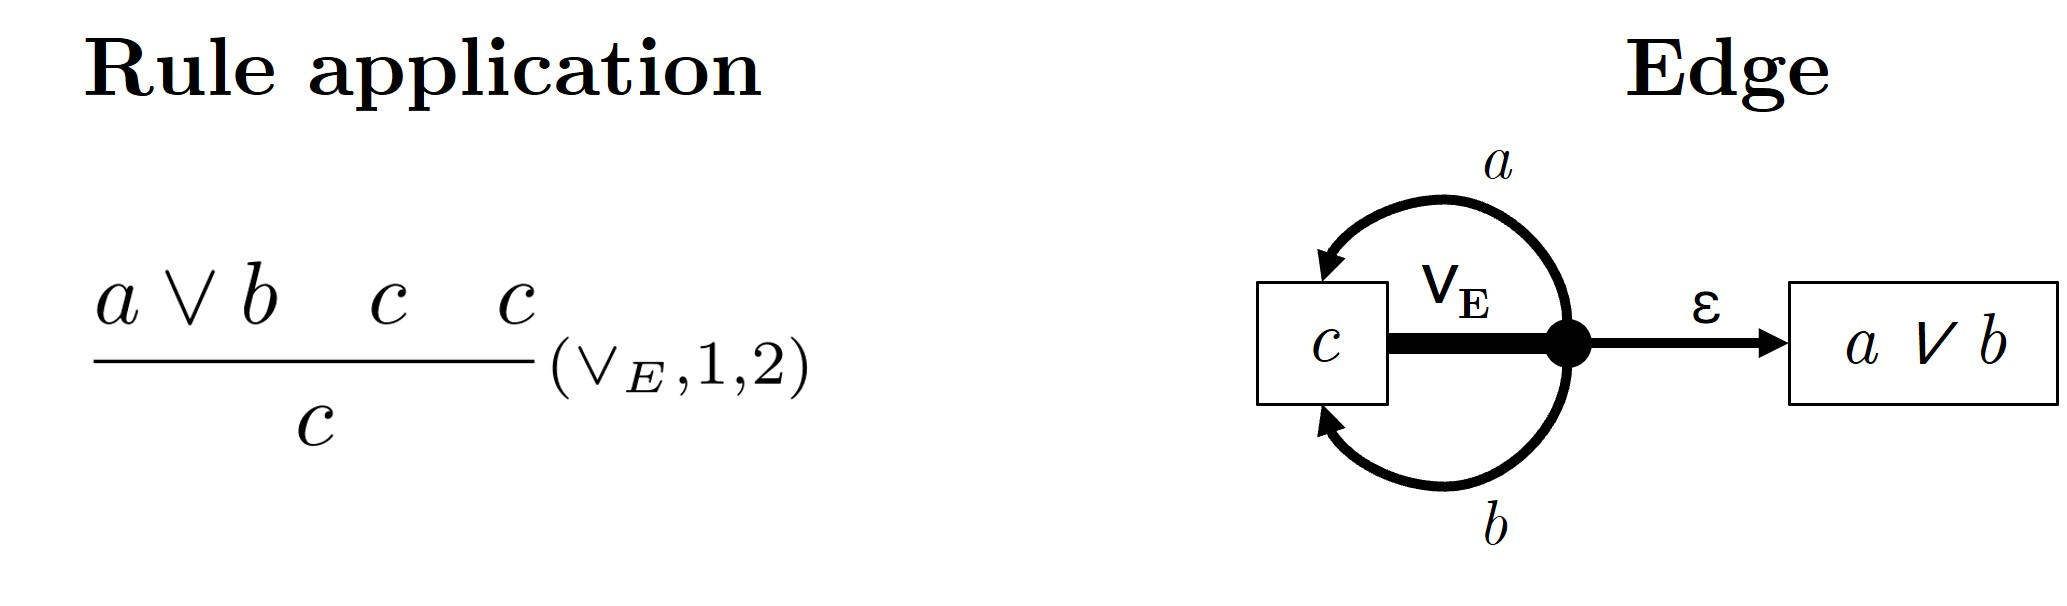
\includegraphics[width=0.8\linewidth]{resources/te-example.jpg}
        \caption{Example of a transition edge.}
        \label{fig:te-ex}
    \end{figure}

We will have the transition: \(T_1 = (\vee_E, \{(a \vee b, \varepsilon), (c, a), (c, b)\})\), and our TG will have this edge: \(E_T = E_T \cup (c, \{T_1\})\). Our edges will always point from the conclusion to its hypotheses. If we are working on FOL proofs, we also need to consider the side conditions as part of the transition. The reason why we are using hypergraphs instead of regular graphs is that some rule applications can have more than one hypothesis, like in the example we showed and we want to map them in the graph.

\vspace{1em}
\textbf{Procedure: }

\begin{enumerate}
    \item First, we initialize our graph by defining the set of possible formulas \(F\) as the union of all formulas in the problem and the initial state. The set of rules \(R\) are the rules presented in Figure \ref{fig:nd-rules}, and the edges \(E_T\) are initialized as an empty set.

    \item We loop through all formulas in \(F\), and for each formula \(f\):

    \begin{enumerate}
         \item We add its negation \(\lnot f\) to \(F\), but only if the expression was not already added as the negation of another expression (to avoid infinite loops). We include negations to support indirect proofs using the Absurdity rule.
         \item If \(f\) is not a literal, we decompose it and add the decomposed formulas to \(F\).
    \end{enumerate}

    Figure \ref{fig:tg-exps} shows an example of the decomposition of the expression \(a \to ( b \land \lnot c)\) 
    \begin{figure}
        \centering
        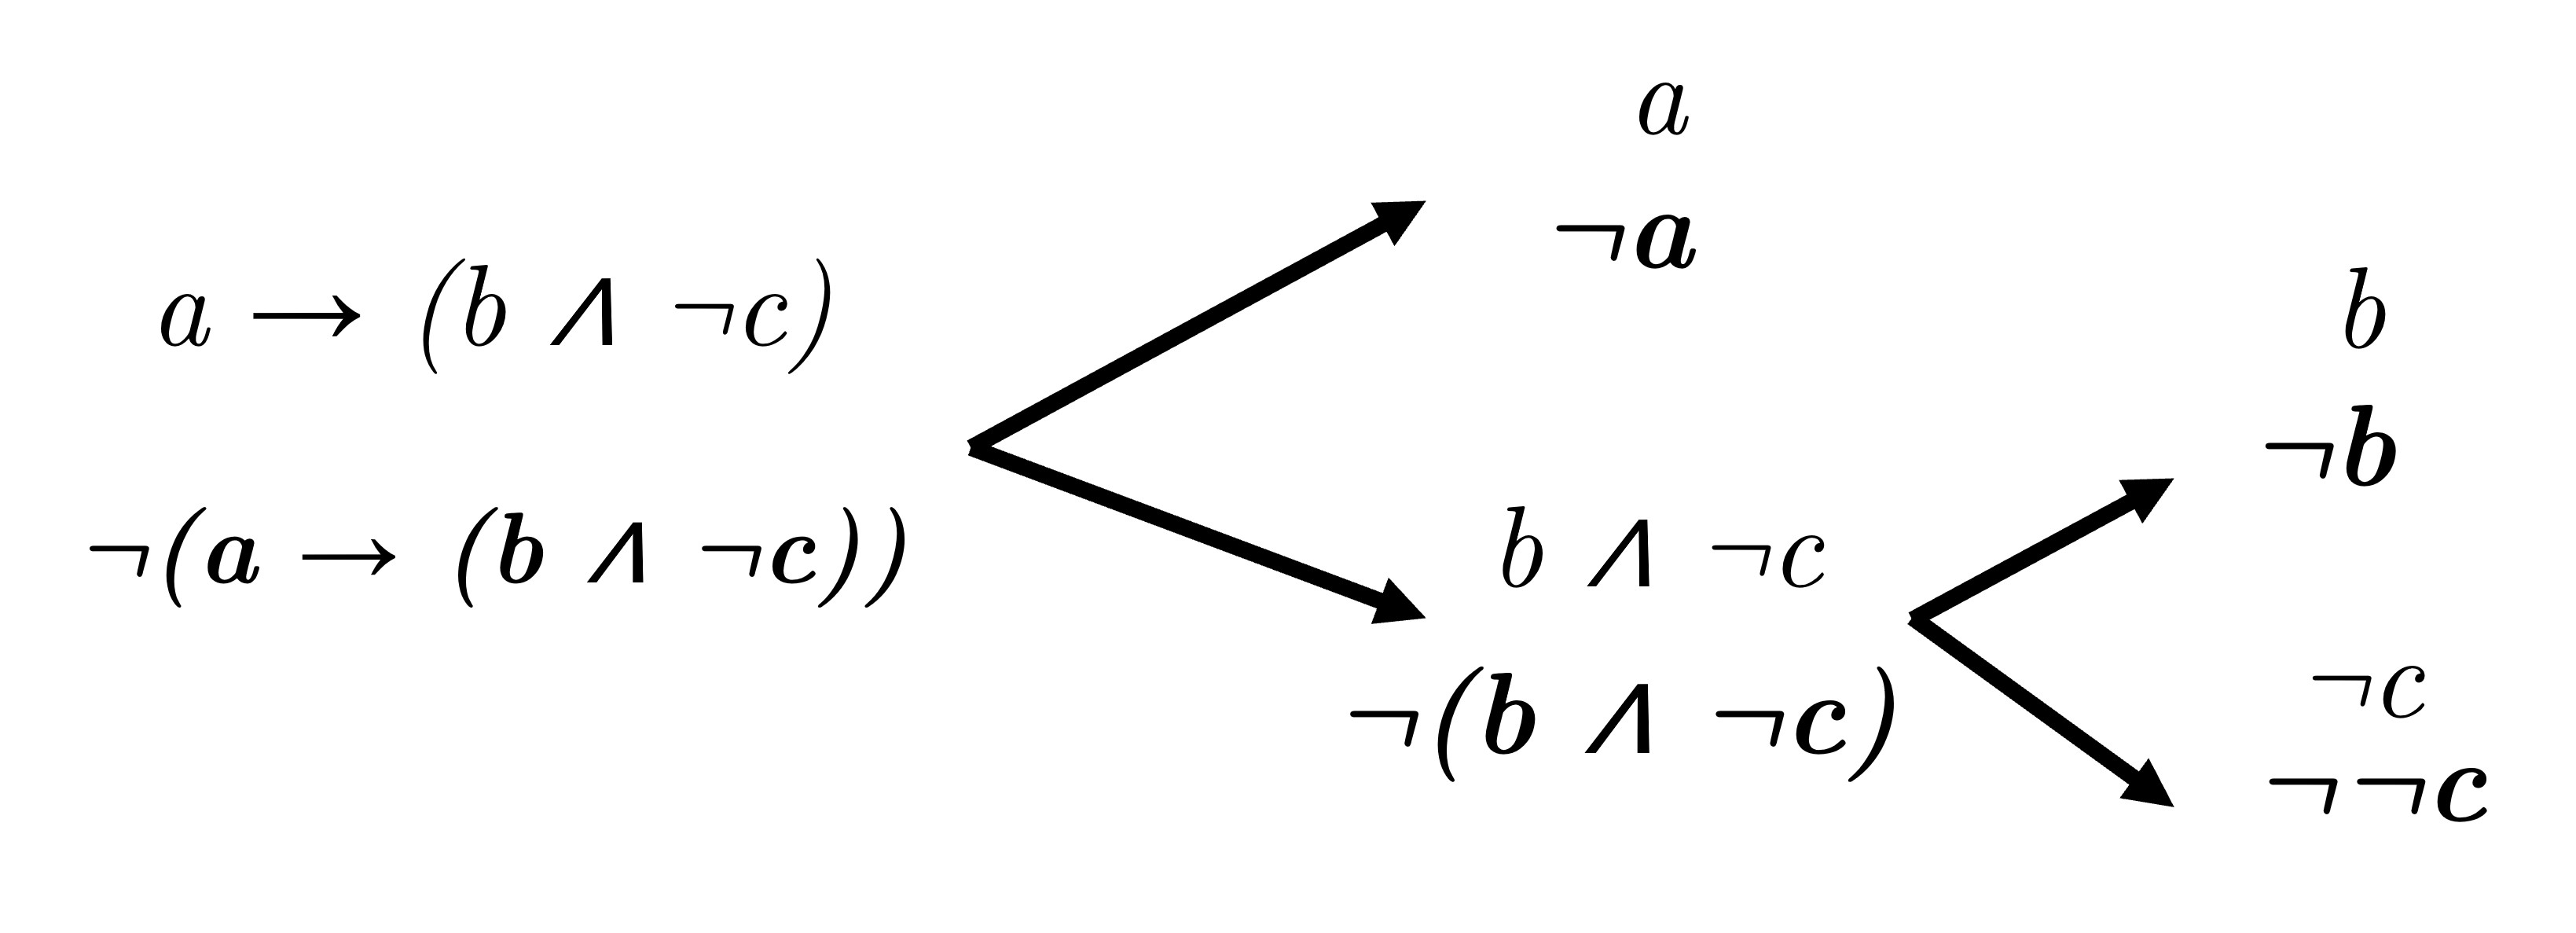
\includegraphics[width=0.6\linewidth]{resources/decomposition.jpg}
        \caption{Decomposition of the expression \(a \to ( b \land \lnot c)\)}
        \label{fig:tg-exps}
    \end{figure}

    So, at the end of this iteration, the set of formulas will be: \(
    F = \{ a \to ( b \land \lnot c), \lnot(a \to ( b \land \lnot c)), a, \lnot a, b \land \lnot c, \lnot(b \land \lnot c), b, \lnot b, \lnot c, \lnot\lnot c \}.
    \)

    \item After computing the formulas that our proof can contain, we select which rules can be applied to each formula. To do that, we loop again through the formulas \(F\), and for each formula \(f\):

       \begin{enumerate}
            \item For each rule \(r \in R\):

            \begin{enumerate}
                \item If the rule is Absurdity, we add a transition edge to the graph, as this rule can be applied to any formula.
                \item Else if the rule is Elimination of Negation and \(\lnot f \in F\), we add a transition edge with that rule.
                \item Else if \(f\) is a conjunction and the rule is Elimination of Conjunction, we add a transition edge with all matching formulas in \(F\). The reason for this is that the Elimination of Conjunction rule can be applied to any formula when there is a disjunction, the same applies to the Elimination of Existential rule.
                \item Else if \(f\) is not a literal and does not match the above rules, we try to match \(f\) with rule \(r\) using its outermost logical symbol. For example, if \(f = a \to b\), it matches the Introduction and Elimination of Implication.
            \end{enumerate}  

            An example of the edges generated for the formula \(a \to b\) is shown in Figure \ref{fig:tg-edges}.
    
            \begin{figure}
                \centering
                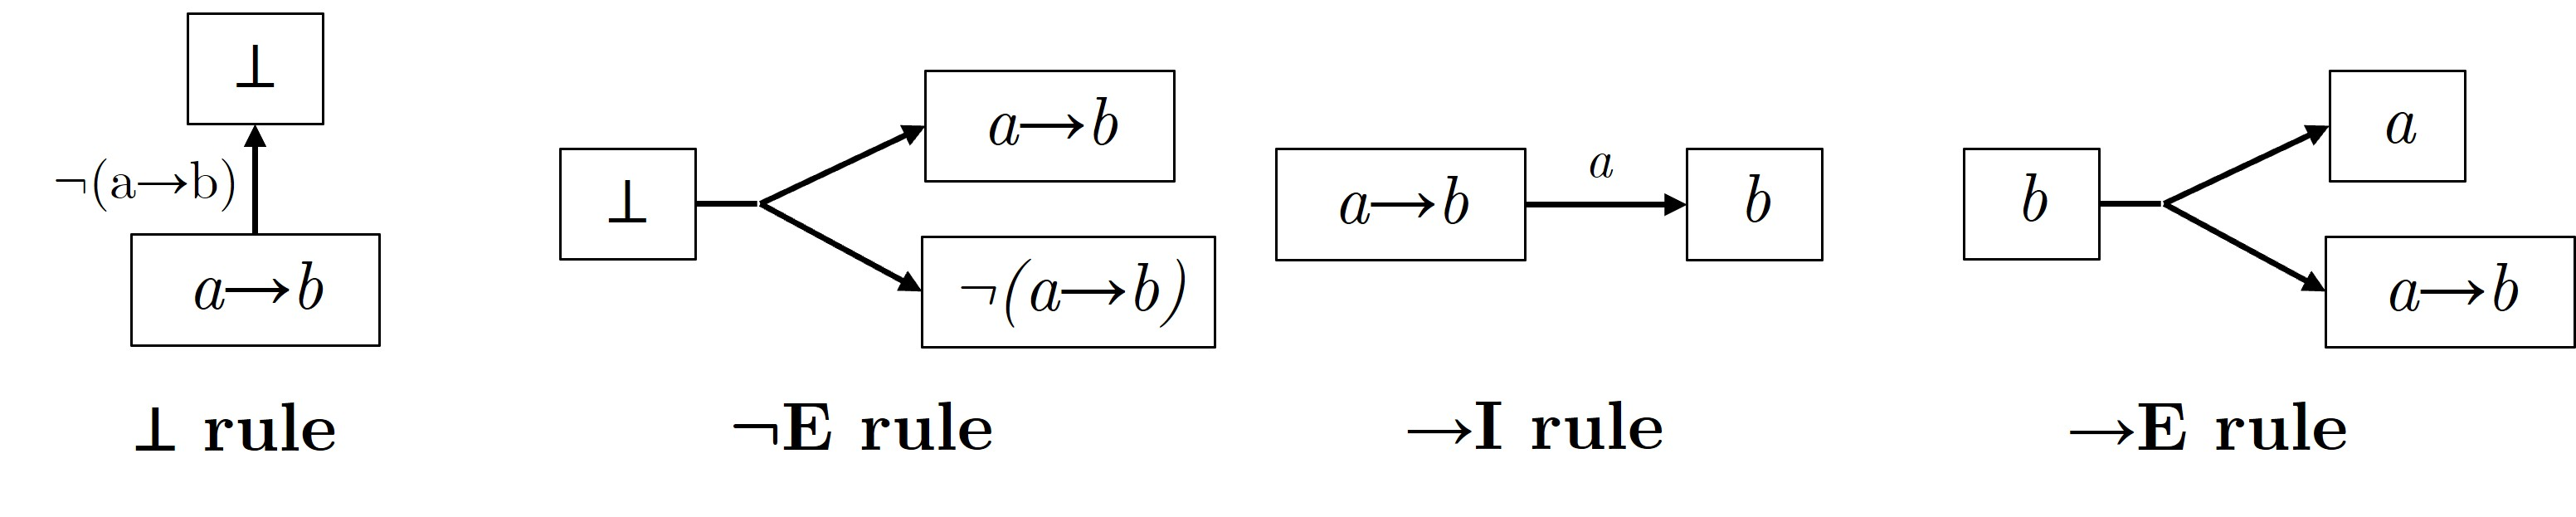
\includegraphics[width=1\linewidth]{resources/tg-edges.jpg}
                \caption{Edges generated for the formula \(a \to b\)}
                \label{fig:tg-edges}
            \end{figure}
    \end{enumerate}    

    As the algorithm considers the deviations taken by the formulas derived in the incomplete proof, it will be able to generate solutions that are more aligned with the student’s reasoning process. Figure \ref{fig:tg-final} shows the final TG for the problem \(\vdash a \to a\), considering all possible formulas and transitions for this problem.

    \begin{figure}
        \centering
        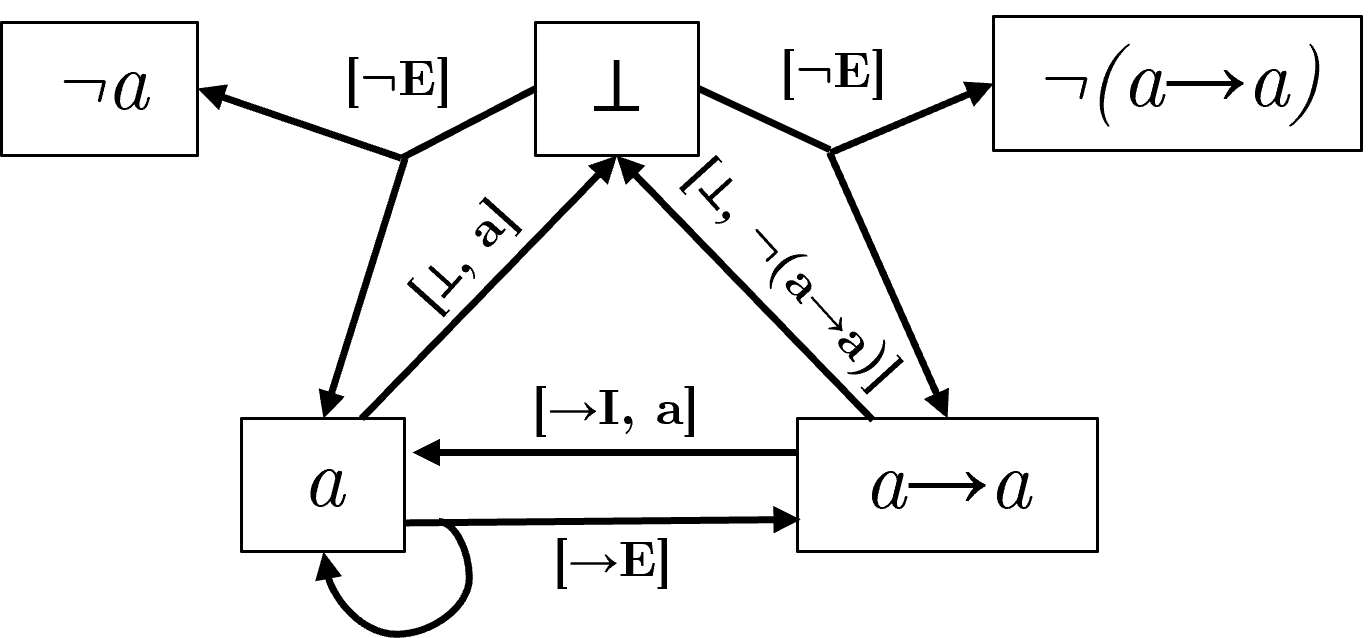
\includegraphics[width=0.6\linewidth]{resources/tg-final.png}
        \caption{Final TG generated from \(\vdash a \to a\)}
        \label{fig:tg-final}
    \end{figure}
\end{enumerate}



\begin{algorithm}
\caption{Transition Graph Construction}
\KwIn{Problem $(\Gamma, \phi)$, Incomplete State $(\Delta, \alpha)$}
\KwOut{Transition Graph $TG = (F, R, E_T)$}

$F \leftarrow \Gamma \cup \Delta \cup \{\phi, \alpha\}$ \tcp*[r]{Initialize formulas}
$E_T \leftarrow \emptyset$ \tcp*[r]{Initialize edges}
$R \leftarrow$ set of inference rules \tcp*[r]{Load rules}

\tcp{Compute formulas}
\ForEach{$f \in F$}{
  \If{$f $was not already added as the negation}{
    $F \leftarrow F \cup \{\lnot f\}$ \tcp*[r]{Add negation for indirect rules}
  }

  Decompose $f$ into parts $S$\;
  $F \leftarrow F \cup S$\;
}

\tcp{Compute transitions}
\ForEach{$f \in F$}{
    \ForEach{$r \in R$}{
      \If{$r$ is the Absurdity rule}{
        $T_e = (r, \{(\bot, \lnot f)\})$\;
        $E_T \leftarrow E \cup \{(f, \{T_e\})\}$\;
      }
      \ElseIf{$r$ is the Elimination of Negation rule and $\lnot f \in F$}{
        $T_e = (r, \{(f, \varepsilon), (\lnot f,\varepsilon)\})$\;
        $E_T \leftarrow E \cup \{(\bot, \{(r, T_e)\})\}$\;
      }
      \ElseIf{$r$ is the Introduction of Conjunction rule and $f$ is a conjunction $(\psi \lor \phi)$}{
        \ForEach{$f_\text{sub} \in F$}{
            $T_e = (r, \{(f, \varepsilon), (f_\text{sub},\psi), (f_\text{sub}, \phi)\})$\;
            $E_T \leftarrow E \cup \{(f_\text{sub}, \{(r, T_e)\})\}$\;
        }
      }
      \ElseIf{$f$ is not a literal and none of the rules above}{
        \If{$r$ matches $f$ based on its main logical symbol}{
          Compute the transition edge and add it to the edge to the graph\;
        }
      }
    }

}
\end{algorithm}



\subsection{State Graph}

The second step is to build the State Graph (SG). To do this, we use the previous TG and the state we want to complete. This could be the original problem or a part of the proof the student did not finish. The SG is similar to the TG, but instead of storing transitions, it stores states. Before we describe the procedure, let us define some key terms:

\begin{definition}[State Graph]
The SG is defined as a quadruple:
\[
SG = (\beta, TG, S_F, E_S),
\]
where \( \beta \) is the initial state, \(TG\) is the Transition Graph, \(S_F \subseteq \mathcal{P}(S)\) is the set of discovered states, and \(E_S \subseteq F \times \mathcal{P}(SE)\) maps each formula \( f \in F \) to a (possibly empty) set of state edges.
\end{definition}

\begin{definition}[State Edge]
A \emph{state edge} is an element of the set
\[
S_E \subseteq R \times \mathcal{P}(S),
\]
where \(R\) is the rule applied, and \(\mathcal{P}(S)\) is the set of possible new states after applying that rule.
\end{definition}

\begin{definition}[Closed state]
A state \(S = (\alpha, \Delta)\) is \emph{closed} if \(\alpha \in \Delta\).
\end{definition}

\vspace{1em}
\textbf{Procedure:}

\begin{enumerate}
    \item The algorithm starts by setting the initial state \(\beta\). This can be the original problem state or the incomplete part of the student's proof. The TG is the one built before. The set of found states \(S_F\) starts with only \(\beta\), and the set of edges \(E_S\) is empty.

    \item Then, we go through each state \(s = (\alpha, \Delta)\) in \(S_F\):

    \begin{enumerate}
        \item If the state is closed, we skip it. There is no need to explore it further, because a valid mark can be assigned to it at this point. Other stopping conditions are needed to avoid very long executions, since the graph can grow very fast. For example, we can set a limit on the number of nodes explored.

        \item Then we use the Transition Graph (TG) to find all rule applications for the formula \(\alpha\). This gives us a set of rule applications. For each transition:

        \begin{enumerate}
            \item We apply the rule to the current state \(s\). If this creates a new state, we add it to \(S_F\). The new state is always constructed based on the current state \(s\), keeping track of the transformations made in previous states.
        \end{enumerate}

        \item Finally, the algorithm combines the rule and the generated states into a state edge \(S_E\), and adds it to the set \(E_S\).
    \end{enumerate}
\end{enumerate}


Figure \ref{fig:st-ex} shows part of the graph for the problem \(\vdash a \to a\). Nodes represent states. Solid borders are closed states and dashed borders are unclosed states. In this example, the state $\{\lnot a, \lnot(a \to a)\}$ cannot be closed because $\lnot a \notin \{\lnot(a \to a)\}$, and $\lnot a$ has no outgoing edges in the TG (Figure~\ref{fig:tg-final}).

\begin{figure}
    \centering
    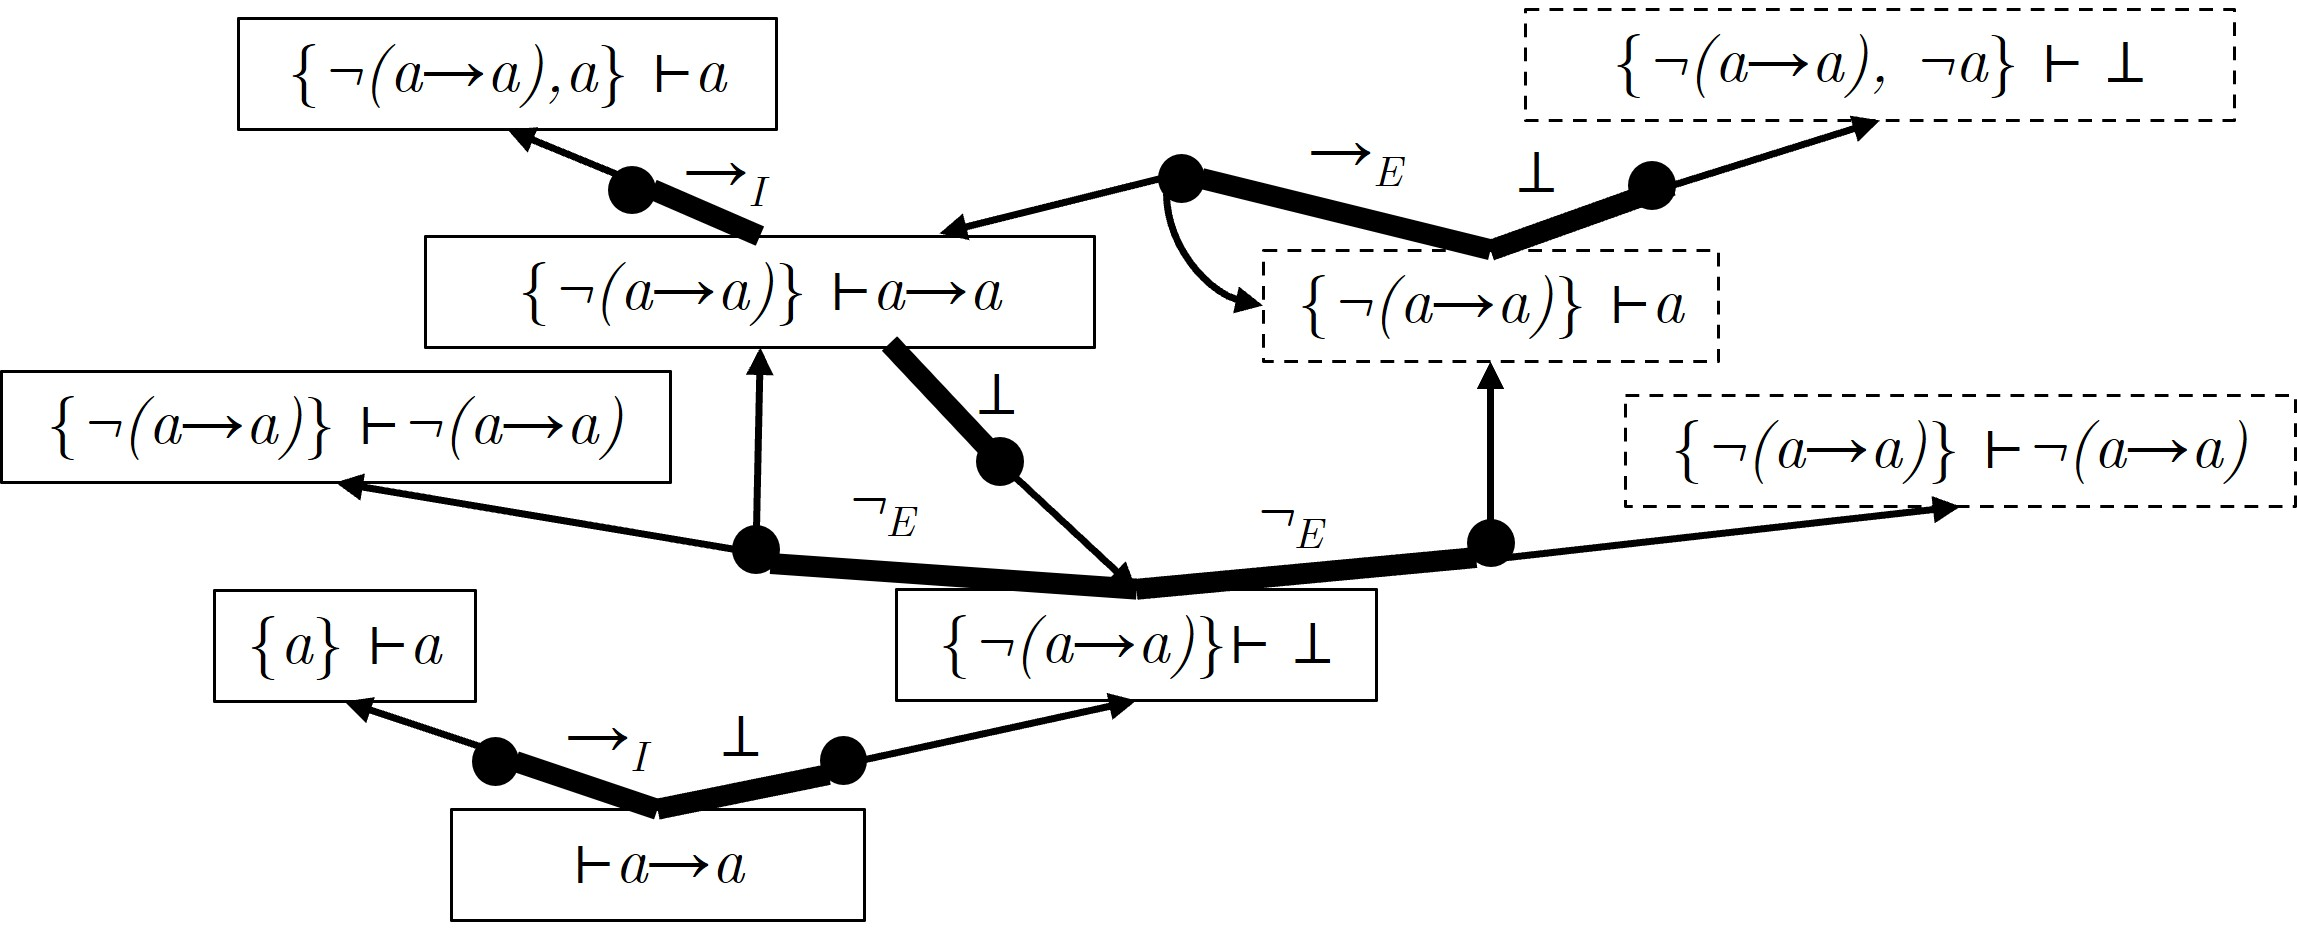
\includegraphics[width=1\linewidth]{resources/sg-gen.jpg}
    \caption{Example of State Graph for \(\vdash a \to a\)}
    \label{fig:st-ex}
\end{figure}

\begin{algorithm}
\caption{State Graph Construction}
\KwIn{Transition Graph $TG$, Initial State $\beta$}
\KwOut{State Graph $SG = (\beta, TG, S_F, E_S)$}

$S_F \leftarrow \{\beta\}$ \tcp*[r]{Initialize set of states}
$E_S \leftarrow \emptyset$ \tcp*[r]{Initialize state edges}

\tcp{Expand states}
\ForEach{$s = (\alpha, \Delta) \in S_F$}{
    \If{$s$ is closed or s}{
        \textbf{continue} \tcp*[r]{Skip closed state}
    }

    \If{stopping condition is reached}{
        \textbf{break} \tcp*[r]{Avoid too many expansions}
    }

    \tcp{Apply rules from TG}
    Get list of rule applications $T$\;

    \ForEach{$(r, t) \in T$}{
        Compute new states $S_r$ from $s$ using transitions $t$\;
    
        $S_E \leftarrow (r, S_r)$\;
        $E_S \leftarrow E_S \cup \{(\alpha, \{S_E\})\}$ \tcp*[r]{Add state edge}
    }

}
\end{algorithm}

\subsection{Trim Graph}

The final stage of our algorithm is to trim the SG and keep only the valid solutions to the problem. In other words, the final trimmed graph will contain only states that lead to a complete and valid proof. To achieve this, we remove unclosed states and extra edges from the SG.

We define two different strategies to trim the graph. Both use a standard graph traversal technique, breadth-first search, to identify which states and edges should be kept. The difference lies in what each strategy prioritizes: the \textbf{Height Trim Strategy} focuses on finding proofs with the smallest height (fewest layers of rule applications), while the \textbf{Size Trim Strategy} aims to find proofs with the fewest total steps (smallest number of rule applications).


\vspace{1em}
\textbf{Height Trim Strategy Procedure:}  
This strategy loops through all closed states and tracks the height needed to reach each one. For every descendant of a closed state, the algorithm continues this tracking process. Because it uses breadth-first traversal, the first time a node is reached, it’s guaranteed to be through the shortest possible path (in terms of height). This makes the strategy efficient.

\vspace{0.5em}
\textbf{Size Trim Strategy Procedure:}  
This strategy also starts from closed states. It updates the size (number of steps) required to reach each ancestor. For each state, it keeps only the edge that leads to a smaller proof. For every descendant
of a closed state, the algorithm continues this tracking process. This process ensures that each state keeps at most one optimal incoming edge, leading to the shortest proof found within the SG's search space. Although slower than the height trim strategy, it finds more concise proofs in terms of rule applications.

\vspace{1em}
Figure~\ref{fig:sg-trim} shows an example of a trimmed SG using the \textbf{Size Trim Strategy}, on the SG shown in Figure~\ref{fig:st-ex}. The states that could not be closed were removed, and the edges coming from higher-level solutions were also trimmed.

\begin{figure}
    \centering
    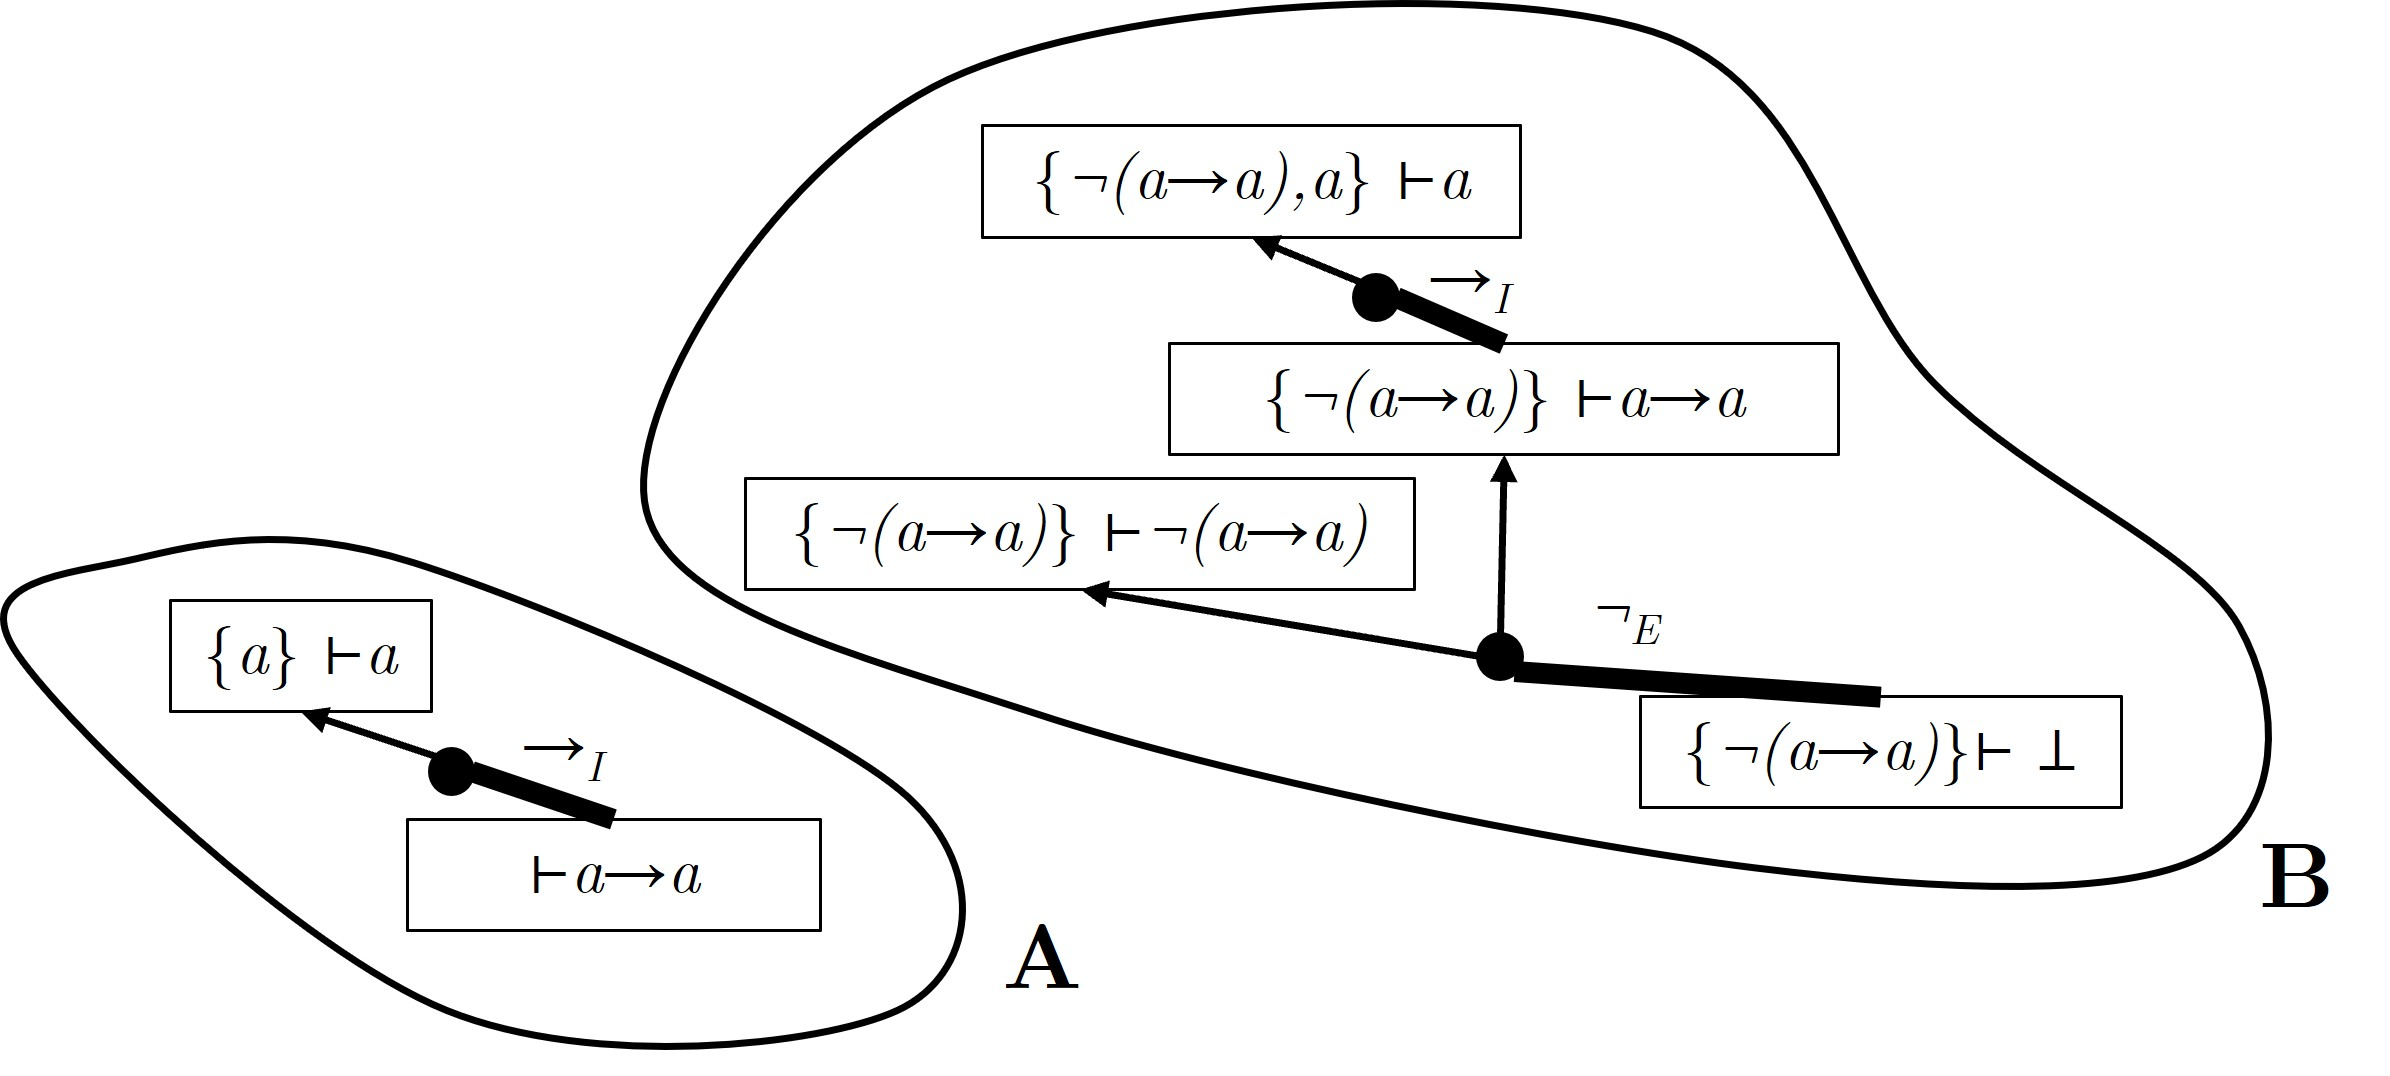
\includegraphics[width=1\linewidth]{resources/sg-final.jpg}
    \caption{Trimmed State Graph showing valid proof paths.}
    \label{fig:sg-trim}
\end{figure}

To check whether a valid solution was found for the full proof, we simply verify if the initial state appears in the trimmed graph. In the example above, the solution corresponds to tree \textbf{A}, as we want to solve the problem \(\vdash a \to a\). That solution is always the smallest in height/size, respectively. With this trimmed graph, we can now generate feedback by querying which states are still missing in the student’s proof. Figures \ref{fig:extract-solution} and \ref{fig:extract-solution2} illustrate examples of how feedback can be generated from the final graph.

In this first example, the student does not know how to proceed after applying the Absurdity rule. By running the algorithm and querying the final graph with the state that is still unsolved, we get a possible solution. This case represents tree \textbf{B} in Figure~\ref{fig:sg-trim}. Knowing the remaining part of the proof, we can generate feedback. For example, we can tell the student to apply the Elimination of the Negation rule using \(a \to a \) and  \(\lnot(a \to a) \) (\textbf{Providing guidance on rule applications}). In this specific case, we cannot give hints about sub-proofs to solve the problem, as the solution is already small. But in some cases where the solution is bigger, we can do that (\textbf{Breaking proofs into smaller sub-proofs}). We can also specify how far the student is from the final proof. In this case, we can say that they are two rules away from completing the proof (\textbf{Indicating the distance to a solution}). Finally, we can also suggest some improvements in the resolution. In this case, the student shifts their solution by applying the Absurdity rule, making it longer. That information can also be extracted from the graph by comparing the smallest proof (the one with the initial state) with the student’s final proof (\textbf{Improvements in the proof}).

 
\begin{figure}
    \centering
    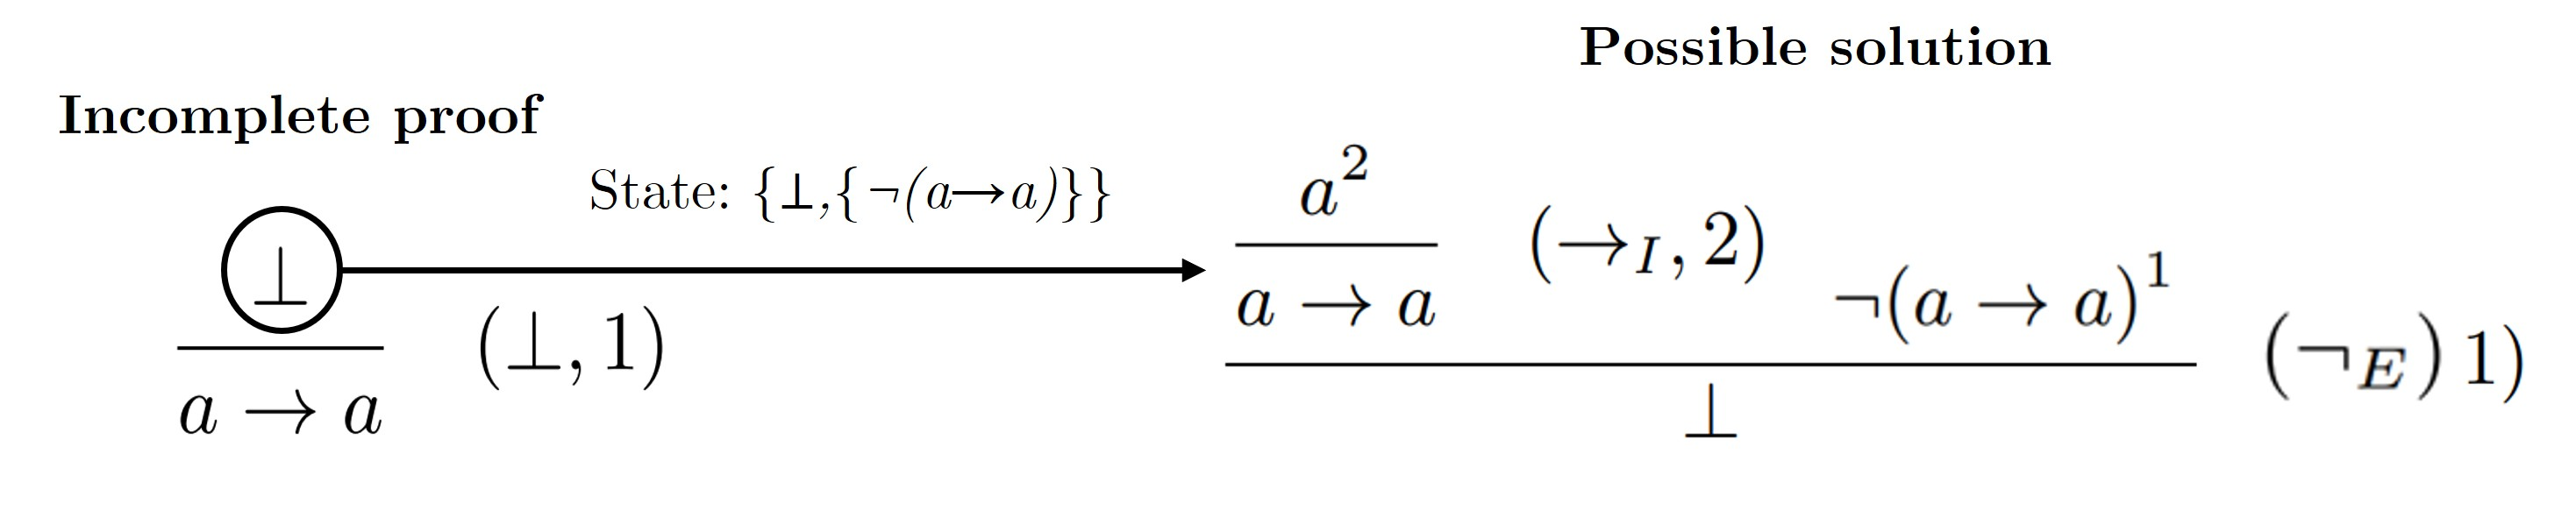
\includegraphics[width=1\linewidth]{resources/trim-pos-feed.jpg}
    \caption{Extracting a solution to produce feedback using an existing state}
    \label{fig:extract-solution}
\end{figure}

In this second example, a solution cannot be found, as the state assigned to the unresolved part of the proof does not belong to the final graph. In this case, we can inform the student that the path they are taking may be too complex, and we can suggest going back \(X\) rule applications until the algorithm finds the correct path again to guide the student. We cannot affirm that there is no solution, because we may not have explored the whole space of possible solutions. In this example, if the student removes the Elimination of Negation rule (one step back), we return to the situation previously presented.

\begin{figure}
    \centering
    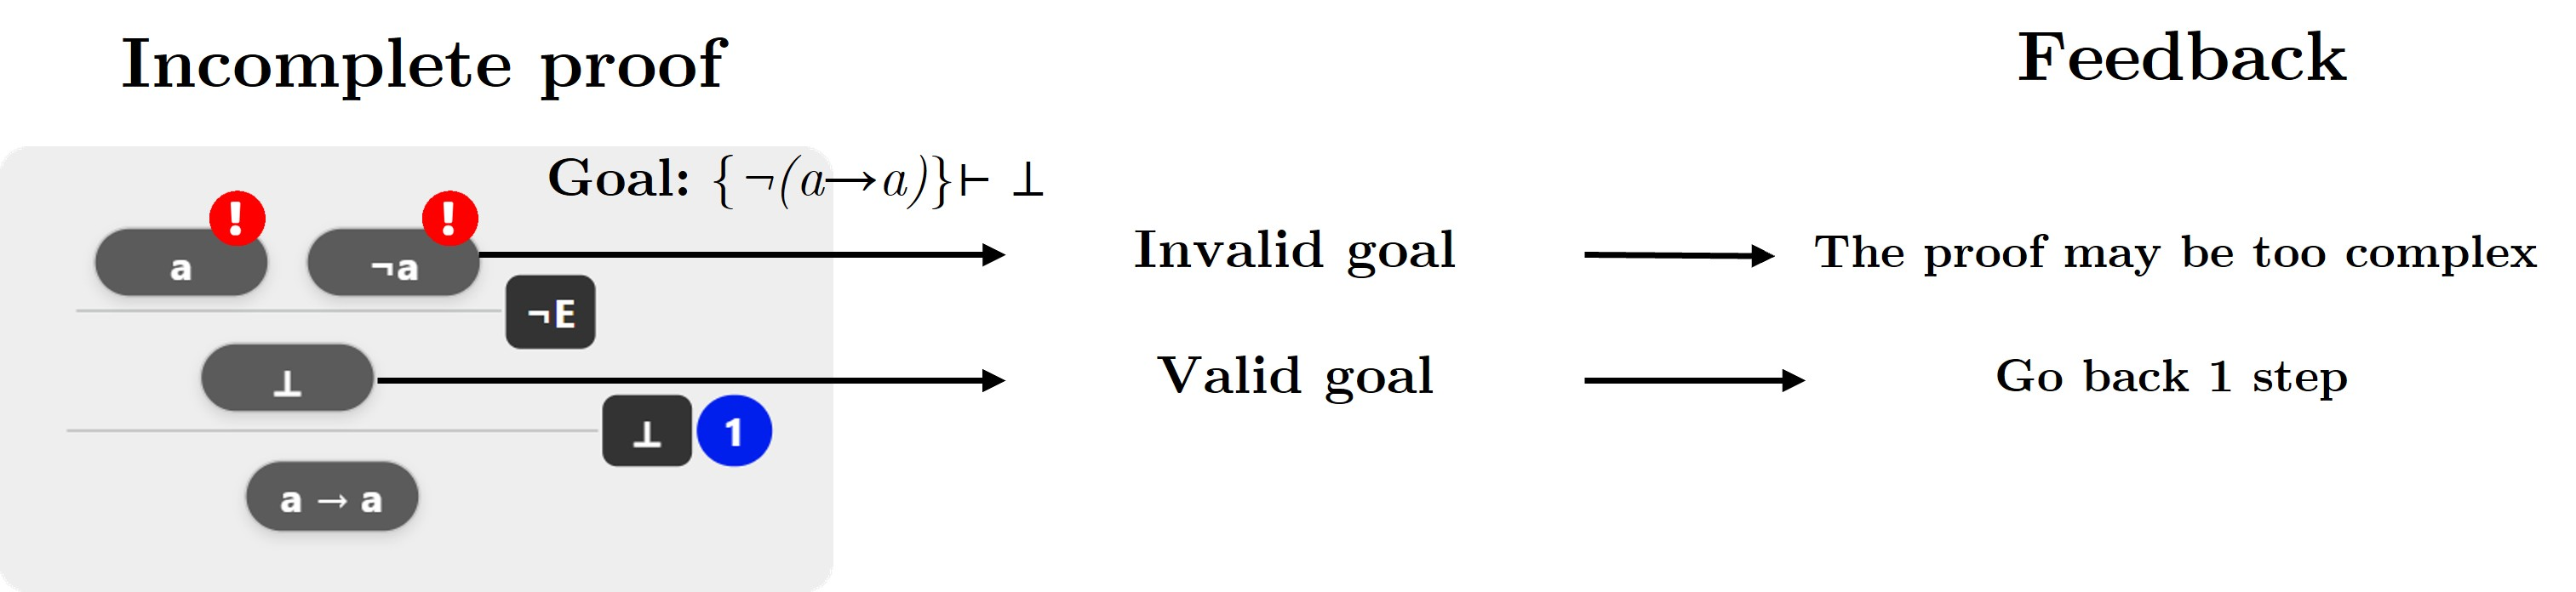
\includegraphics[width=1\linewidth]{resources/trim-neg-feed.jpg}
    \caption{Extracting a solution to produce feedback using a non-existing state.}
    \label{fig:extract-solution2}
\end{figure}

These methodologies can also be used to assess exercises. For example, by computing how far the student’s resolution is from a possible solution if the problem remains unsolvable, or how far it is shifted from the best solution. In some cases, based on the size of the explored solution space, we can say that the student overcomplicated the resolution.

\section{Limitations}
The algorithm was developed for pedagogical purposes, so efficiency in proof generation was not our main focus. It can generate solutions for most exercises used in teaching environments but is more limited when searching for solutions in FOL proofs, as the solution space is infinite. Our algorithm is sound: if it finds a solution, it is definitely correct. This is guaranteed by the TG, which only generates valid transitions for each formula, and by the SG, which ensures that all leaves in the proof are correctly closed.

Regarding completeness, our algorithm is not complete because it can only find solutions up to a certain depth. Some proofs generate infinite graphs, so a solution may not be found. In most cases, this is not a problem, as we aim to find direct proofs. If a student’s proof deviates too much from the solution, it is not useful to provide feedback on that solution because the student is overcomplicating the problem. For example, if a teacher sees that a student is still working on a problem that can be solved in 10 steps, but the student’s current resolution already has 50 steps, even if a solution exists following the student’s approach, is it helpful to give feedback on it? Will the student really learn from that? 


\section{Conclusion}
Conclusion

\bibliography{bibliography}
\end{document}
